\section{Model-based Reinforcement Learning}
\label{sec:model_based}
\textit{This section reviews the lecture slides 11 and 12.}
\begin{itemize}
	\item We have seen that given the environment dynamics, we can find the optimal policy by dynamical programming. All the methods after that purely learned from interactions. We now want to take a step in between and try to learn the model dynamics itself, $p(s'|s,a)r(s,a,s')$. If we have that, we could plan by simulating in our learned model.
	\item There are several benefits of this approach:
	\begin{itemize}
		\item We don't require interactions with the environment, but can generate new data from simulation. This is especially helpful when real-time data is expensive (whether in time, computational resources, etc.) as in real-life robotic systems (takes a long time for a single rollout)
		\item We can obtain probability distributions which tell us how likely we end up in a state when we take a certain action. This can be very helpful in some cases, as e.g. in the (slippery) cliff world example, we would know how likely it is that we actually fall of the cliff even if we take the right action. 
	\end{itemize}
	However, when these things are not required, model-free methods mostly work better and/or are computationally cheaper/simpler. Furthermore, we prevent any bias we might get when our model is inaccurate.
	\item In general, we distinguish between three types of systems we can have that tries to imitate the real environment:
	\begin{itemize}
		\item A \textbf{full} or \textbf{distributional model} is a full description of all transition probabilities and rewards. 
		\item A \textbf{sample} or \textbf{generative model} can be viewed as a black-box simulator, where given any state $s$ and action $a$, it can sample a reward $r_t$ and a next state $s'$.
		\item A \textbf{trajectory} or \textbf{simulation model} can simulate whole episodes, but is not able to start at any state and action. This is for example the case for a physical model where we cannot start with an arbitrary velocity.
	\end{itemize}
	These three models can be seen as generalization steps. The most limited implementation is the trajectory one. If we provide the ability of changing the start state to any arbitrary state, we arrive at the generative model. Adding the probabilities $p(s',r|s,a)$ gives us in the end the distributional model.
	\item There are several ways of implementing this. We will consider here a simple method, called Dyna
\end{itemize}
\subsection{Dyna-Q}
\begin{itemize}
	\item Dyna makes two assumptions of the environment:
	\begin{enumerate}
		\item Our environment is deterministic, meaning that any transition probability are either 1 or 0. 
		\item The state and action space is discrete and limited, so that we can store it in a tabular setting.
	\end{enumerate}
	Note that we can relax the first requirement slightly by storing e.g. how often we came from one state-action pair to another state.
	\begin{figure}[ht!]
		\centering
		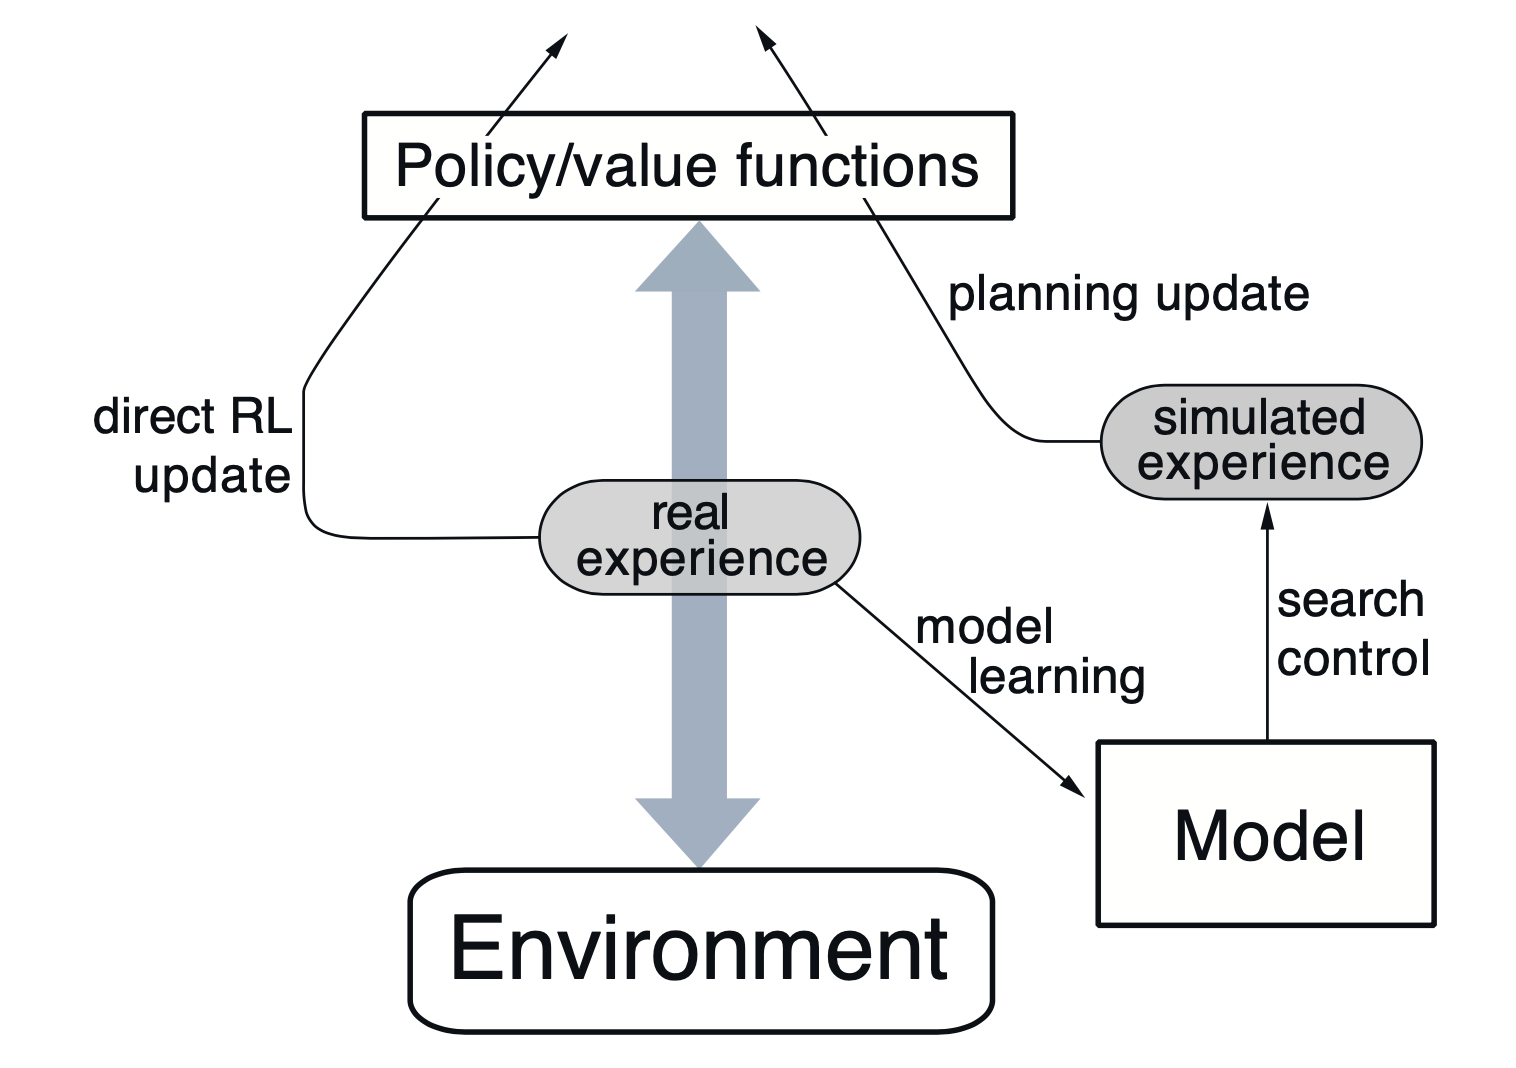
\includegraphics[width=0.4\textwidth]{figures/rl_model_based_dyna_Q.png}
		\caption{Real experience is generated by the interaction of the agent (according to the policy) and the environment. This real data is used to update our policy (direct RL), but at the same time update our model, from which we can generate new samples to learn from (indirect RL).}
		\label{fig:rl_model_based_dyna_Q}
	\end{figure}
	\item The general overview of the idea is shown in Figure~\ref{fig:rl_model_based_dyna_Q}. We have two source from which we train our policy and/or value function: direct and indirect. The samples from the real environment are used to perform "direct Reinforcement Learning" as we use the actual samples to learn. At the same time, we use the real samples to update our model, and can generate from there as many samples as we want.
	\item Written down as an algorithm, we arrive at Figure~\ref{fig:rl_model_based_dyna_Q_algorithm}. The parameter $n$ which specifies how often we train from the simulated/learned model compared to the real environment, is a hyperparameter and depends on the access of the environment (how expensive is it, etc.). However, it is usually $n\gg 1$.
	\begin{figure}[ht!]
		\centering
		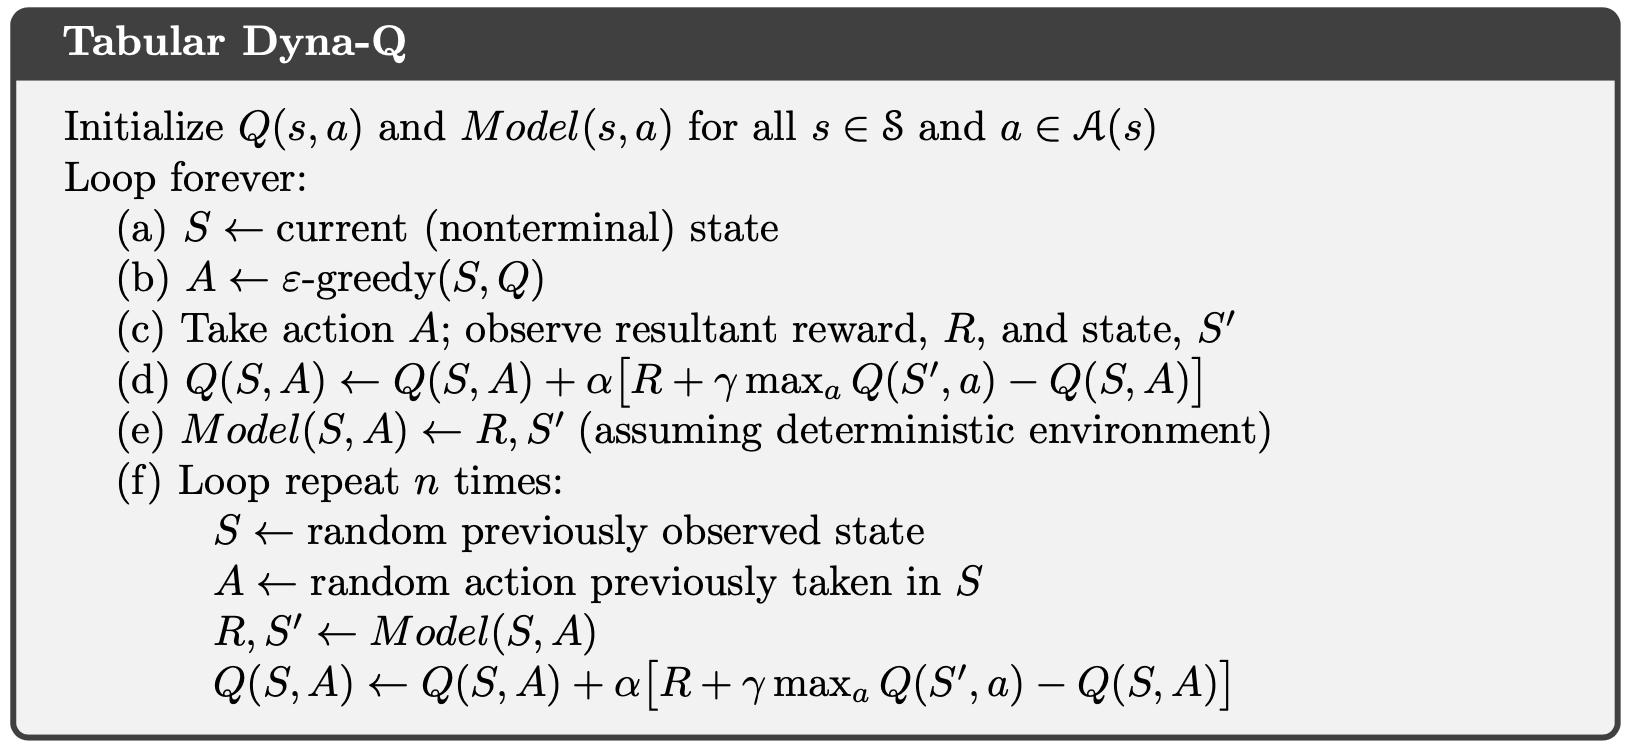
\includegraphics[width=0.65\textwidth]{figures/rl_model_based_dyna_Q_algorithm.png}
		\caption{Example implementation of the algorithm of Dyna-Q. We use a tabular-based setting to store transition and rewards. Note that we will discuss the design choices in this part more in detail.}
		\label{fig:rl_model_based_dyna_Q_algorithm}
	\end{figure}
	\item Looking at Figure~\ref{fig:rl_model_based_dyna_Q_algorithm}, we see that there are still quite a few design decisions to make, which we will go through step-by-step:
	\begin{enumerate}
		\item Step (e) - How do we learn our model?
		\item Step (f) - When should we use our simulated environment? Can we also use it somewhere else than the update step?
		\item Step (f) loop - Which state and action should we choose to update?
		\item Step (f) loop - How do we update e.g. our values or policy?
	\end{enumerate} 
\end{itemize}
\subsubsection{How to learn the model}
\begin{itemize}
	\item As mentioned previously, Dyna uses a tabular setting to learn the model. Hence, we have a table over state and actions, where an entry contains the information of the next state and reward
	\item In case we have stochastic transitions, we have to slightly adjust our table. We now create a table over $(s,a,s')$ where we store how often we experienced this transition, and what reward we got. In case we also have stochastic rewards, we need to extend the table further.
	
	When sampling, we first have to normalize the probabilities for every $s'$ (and $r$) to occur when $(s,a)$ is given, and finally sample from this distribution.
	
	An example table is shown below
	\begin{table}[ht!]
		\centering
		\begin{tabular}{c|cc}
			& \textit{State 1} & \textit{State 2}\\
			\hline
			\textit{State 1, Action 1} & $\eta_{111}=1, r_{111}=2$ (50\%) & $\eta_{112}=1, r_{112}=-1$ (50\%)\\
			\textit{State 1, Action 2} & $\eta_{121}=5, r_{121}=5$ (100\%) & $\eta_{122}=0, r_{122}=0$ (0\%) \\
			\textit{State 2, Action 1}  & $\eta_{211}=4, r_{211}=-4$ (80\%) & $\eta_{212}=1, r_{212}=2$ (20\%)  \\
			\textit{State 2, Action 2} & $\eta_{221}=4, r_{221}=-2$ (40\%) & $\eta_{222}=6, r_{222}=1$ (60\%) \\
		\end{tabular}
		\caption{Example table for stochastic transitions and deterministic rewards.}
	\end{table}
\end{itemize}
\subsubsection{What to update}
\begin{itemize}
	\item To prevent that we spend too much computational effort on state-action pairs that are not relevant for the current/optimal policy, we should make smarter selections
	\item One approach is \textbf{prioritized sweeping} where we prefer these state-action pairs that lead to a state for which we just have experienced an update (whether with real or simulated experience)
	\begin{itemize}
		\item The priority in the queue is given by the TD error we would get at the time we add the state in the queue. This supports that states with high errors, i.e. wrong estimates, are updated first.
		\item To limit the queue, we can define a threshold $\theta$ over which the TD error has to be to add a state in the queue
		\item In the simulation step (indirect RL), we perform updates based on the queue until either the queue is empty, or we reached a maximum of $n$ steps. If the queue is non-empty, it is kept for next iteration as well.
		\item For this model, we require at least a sample/generative model because we need to be able to start at any state-action pair
		\begin{figure}[ht!]
			\centering
			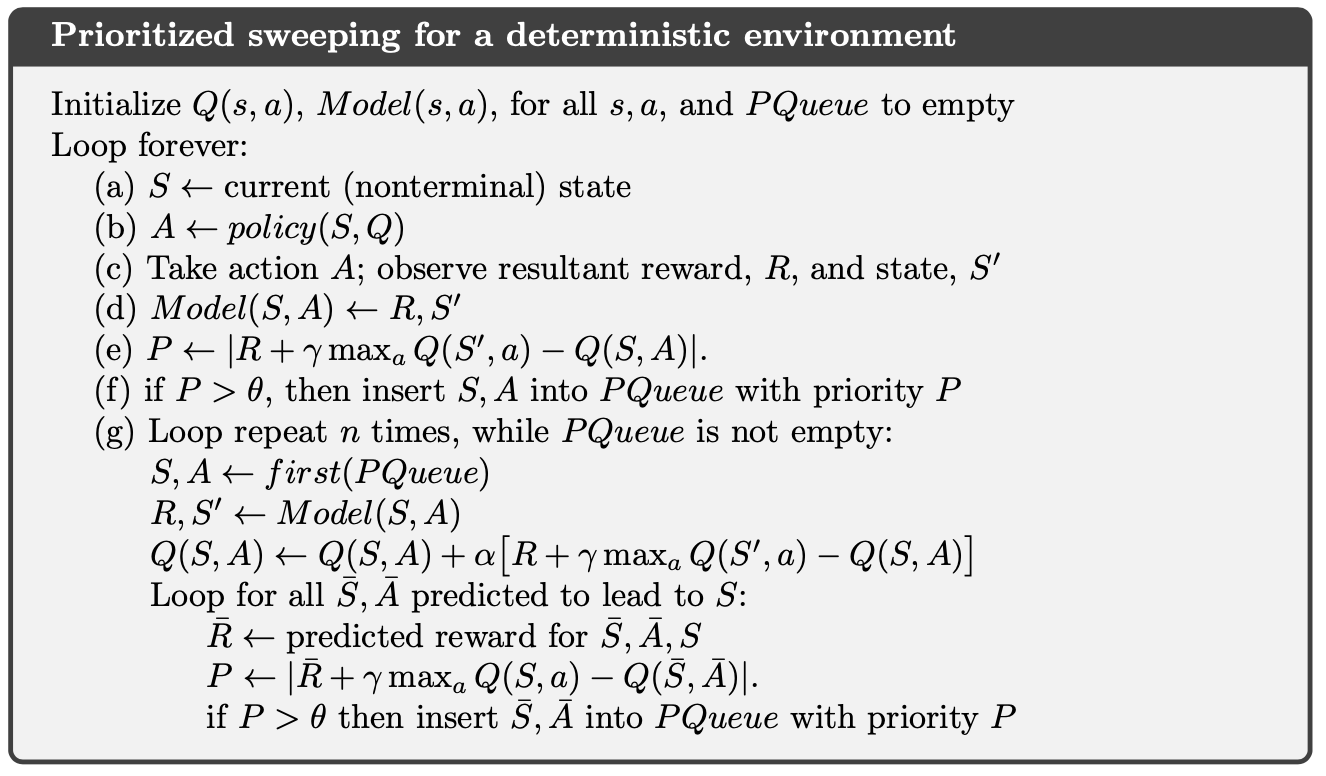
\includegraphics[width=0.5\textwidth]{figures/rl_model_based_dyna_prioritized_sweeping.png}
			\caption{Algorithm of Prioritized Sweeping.}
		\end{figure}
	\end{itemize}
	\item An alternative is performing \textbf{trajectory sampling} where we start from the start state (or sample one if multiple exist), and follow our current policy. 
	\begin{itemize}
		\item While updating the more frequently visited states, we have the disadvantage of limited exploration because we highly focus on states of our distribution
		\item Hence, if we have a (close to) deterministic environment, trajectory sampling might work well, but in a stochastic environment where we continuously have to explore, it might perform worse than uniformly sample any state-action pair 
		\item For this method, we only require a trajectory model, making it less complex
	\end{itemize}
\end{itemize}
\subsubsection{How to update}
\begin{itemize}
	\item For updating our $q$/$v$/policy, we can use any of the methods we have discussed before. 
	\item However, remember that for some methods like dynamic programming, we can make use of the model dynamics. Nevertheless, this might not be the most efficient computation, especially when we have many possible next steps. Remember that we have to take \underline{all} next states into account for dynamic programming, although some can be neglected if we have a small weight on them. 
	\item In addition, we would require the full/distributional model to perform these kind of updates, whereas the others either work with generative or trajectory models
\end{itemize}
\subsubsection{When to plan}
\begin{itemize}
	\item Currently, we only use the environment to generate new samples for training
	\item Knowing the system dynamics can however be valuable in more than this situation. For example, we can easily plan ahead by trying out different actions, and observing the reward in simulation. Afterwards, we take the actions in real-world which gave the best result in the simulation
	\item This idea is used in Monte Carlo Tree Search algorithms, which we will discuss in more detail in Section~\ref{sec:MCTS_Alpha_Go}. 
\end{itemize}
\subsection{Model-based policy search}
\begin{itemize}
	\item In the previous discussion, we mainly focused on value-based updates. However, we could of course use policy-based methods as well.
	\item Again, the decision of whether to use policy-based or value-based methods is based on multiple decisions. For example, if we need to learn a stochastic policy, or we have continuous actions, then we might want to use policy-based methods. In the case that we have discrete actions and aim for learning a deterministic, greedy policy, value-based methods are more suited because for policy gradient we require the policy to be smoothly changable/differentiable.
	\item Let's assume that the reward is known for now (e.g. we have defined the reward for a problem by our own). Then, we could reformulate the transition function as:
	$$s_{t+1} = f(s_t, a_t) + w$$
	where $f(s_t, a_t)$ is a deterministic function that maps a state-action pair to a new state, and $w$ is additive noise (e.g. Gaussian for continuous states). To ensure this formulation to work well, we would require a mostly deterministic environment, as otherwise $f(s_t, a_t)$ cannot model the different outcomes.
	\item We can then train by
	\begin{enumerate}
		\item Use any model-free policy-based approach (e.g. TRPO or DDPG) to learn from the real world.
		\item Use the extra information from the environment, e.g. for richer gradient information
		\begin{itemize}
			\item As we now model the transition function $s_{t+1}\approx f(s_t, a_t)$, we know how the next state will change if we change our parameters.
			\item This allows us to look at the gradients over $s'$ and $a$, and find the best action more easily
			\item When we perform backpropagation through $v_{\theta}(s_t)$, we can (instead of sampling) also derive rewards because they are a simple function depending on $s_{t+1}$, or in $f(s_t,a_t)$. Hence, we can write:
			$v_{\theta}(s_t)=\nabla_{\theta} r_{t+1}+\gamma \nabla_{\theta} r_{t+2}+...$
		\end{itemize}
	\end{enumerate}
\end{itemize}
\subsection{Monte-Carlo Tree Search and Alpha Go}
\label{sec:MCTS_Alpha_Go}
\begin{itemize}
	\item In Section~\ref{sec:value_based_approximation}, we have seen that to learn a value function for problems with very large state space, we can approximate our $q$-function by e.g. a neural network. However, these approximations will always contain a certain amount of noise/inaccuracy.
	\item An alternative approach is to learn $q_{\pi}(s,a)$ \underline{online}. The simplest approach, when we have given our model, is to perform a couple of rollouts from the state $s_t$ with our current policy $\pi$. $q_{\pi}(s,a)$ can then be estimated by the mean of the experienced returns $G_t$.
	
	Playing the best action based on this estimate (e.g. estimated $q_{\pi}(s_t,a_1)$, $q_{\pi}(s_t,a_2)$, etc.) is guaranteed to be at least as good as $a\sim \pi(s)$ as if $\pi$ was the optimal policy, $a$ will also be the argmax of the estimate (in expectation).
\end{itemize}
\subsubsection{Monte-Carlo Tree Search}
\begin{itemize}
	\item If we have given a full model description including the dynamics, we could simply expand the previous approach by taking all possible futures into account. However, this is less likely to work for games like Go because there are a huge number of possible outcomes (a full game tree has about $10^{170}$ different states). 
	\item Nevertheless, a lot of this computation might not be necessary. Instead, we can focus on the most likely subtree which only contains a small selection of possible outcomes. This leads us to the Monte-Carlo Tree Search algorithm
	\item In MCTS, we build a tree incrementally by performing 4 steps for $n$ steps (limited by computational resources, time, etc.), visualized in Figure~\ref{fig:rl_model_based_MCTS}:
	\begin{enumerate}
		\item \textbf{Selection}
		
		Given a subtree, we need to decide at which point we want to expand it. This is defined by our \textit{tree policy} $\pi_{\text{tree}}$, and can be for example the upper confidence bound (similarly to choosing the next action in a bandit setting):
		$$\pi_{\text{tree}}(s)=\arg\max_{a} \left[Q(s,a)+c\sqrt{\frac{\ln N(s)}{N(s,a)}}\right]$$
		with $N(s)$ as the number of visits in $s$, and $N(s,a)$ the number of times we took $a$ in $s$. We continue our policy until we end up at a leaf node.
		\item \textbf{Expansion}
		
		After deciding at which node we want to "grow" the tree, we need to expand it. This means that we add a new leaf, which is an action in case of $q$, or a state in case of $v$ (we always add a state-action pair, just ordering is different). We initialize it with the values $N(s)=0$, $N(s,a)=0$ in case of UCB.
		\item \textbf{Simulation}
		
		From the newly added node, we perform a rollout. This means that starting from the leaf node, we interact with the environment according to the current policy $\pi$ until terminating. 
		\item \textbf{Backup}
		
		After finishing simulation, we update our estimates based on the newly observed return. Note that we update the $q$/$v$-values for each node which led to the leaf, while taking a possible discount factor $\gamma$ into account. In case of UCB, this means that we increase $N(s)$ and $N(s,a)$ by one, as well as adding a new point to $Q$ for averaging (e.g. use running average).
	\end{enumerate}
	\begin{figure}[ht!]
		\centering
		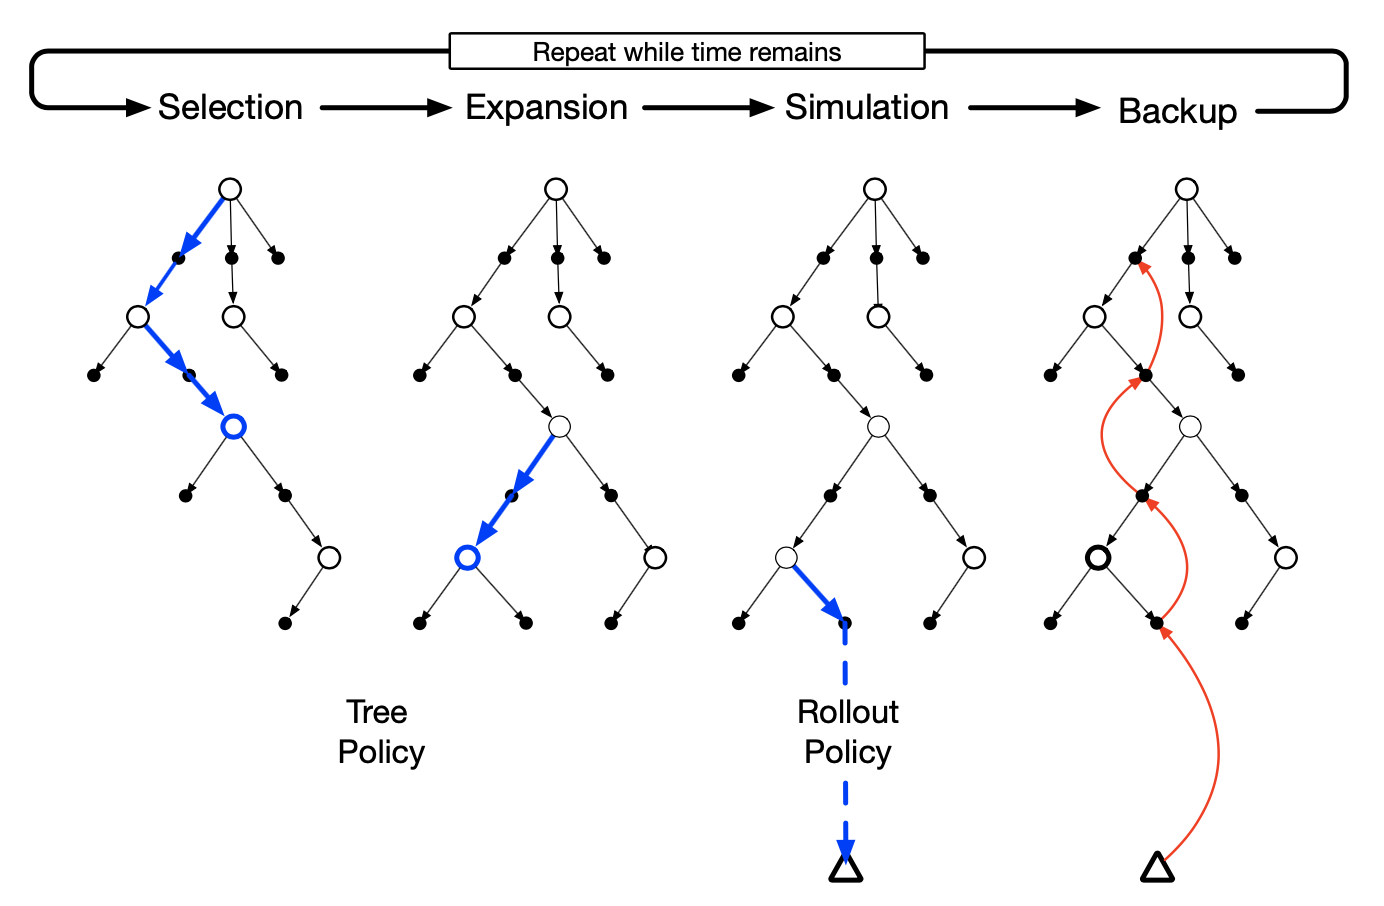
\includegraphics[width=0.6\textwidth]{figures/rl_model_based_MCTS.png}
		\caption{Visualization of the four steps in MCTS: Selection, Expansion, Simulation, Backup.}
		\label{fig:rl_model_based_MCTS}
	\end{figure}
	\item Note that we have seen two requirements of MCTS along the way: (1) we need a generative model where we can start at any $(s,a)$. Alternatively, if our environment is deterministic, we can also make trajectory models working by playing the same actions again from the top. (2) we assume $q(s,a)$ to be storable in a table
	\item If we want to use MCTS for planning, we can choose our our policy based on $\pi(a|s)\propto N(s,a)^{1/\tau}$. Note that we don't take the policy according to the $q$ values because they are estimates, and potentially very noisy as we have different amount of samples for each action.
	\item After taking a step, we can reuse the selected branch of the tree, and don't have to start from scratch again
\end{itemize}
\subsubsection{AlphaGo Zero}
\begin{itemize}
	\item For estimating the $q$-values, MCTS uses full Monte Carlo samples. However, we know that we can also use TD learning for it, meaning we bootstrap our estimates. Using this idea, two separate networks were used in Alpha Go: a policy network $\pi_{\theta}(a|s)$, and a value network $v_{\theta}(s)$
	\item We can now look at the changes AlphaGo makes in the MCTS algorithm:
	\begin{enumerate}
		\item \textbf{Selection}
		
		We define our tree policy as:
		$$\pi_{\text{tree}}(a|s)=\arg\max_a \left[Q(s,a)+cU(s,a)\right], \hspace{5mm}U(s,a)=\frac{\pi_{\theta}(a|s)}{1+N(s,a)}$$
		Note that this is a solution found empirically as we sum $q$-values and probabilities.
		
		\item \textbf{Expansion}
		
		When reaching a leaf node, we evaluate the value network $v_{\theta}(s)$ for this specific state, and expand the state by all its possible actions.
		
		\item \textbf{Simulation}
		
		In the original AlphaGo, we randomly choose between using $v_{\theta}(s)$, or simulating by performing a rollout. However, in the newer version AlphaGo zero, we fully rely on $v_{\theta}(s)$.
		
		\item \textbf{Backup}
		
		Using $v_{\theta}(s)$, we update all $q$ values above.
	\end{enumerate}  
	\item Our policy network $\pi_{\theta}$ limits our search in width because we select values based on its prior. The value network $v_{\theta}(s)$ limits the search in depth because we don't have to sample anymore.
	\item This approach is working well, if we have (1) a discrete state space, (2) a fully observable environment, and (3) a deterministic environment.
	\item We train the network by self-play. The policy network tries to predict the outcome of the tree search (how often will we choose action $a$ at state $s$), and the value network tries to predict the return we get after the full rollout. See Figure~\ref{fig:rl_model_based_alphago_zero_selfplay} for a visualization of the self-play learning.
	\begin{figure}[ht!]
		\centering
		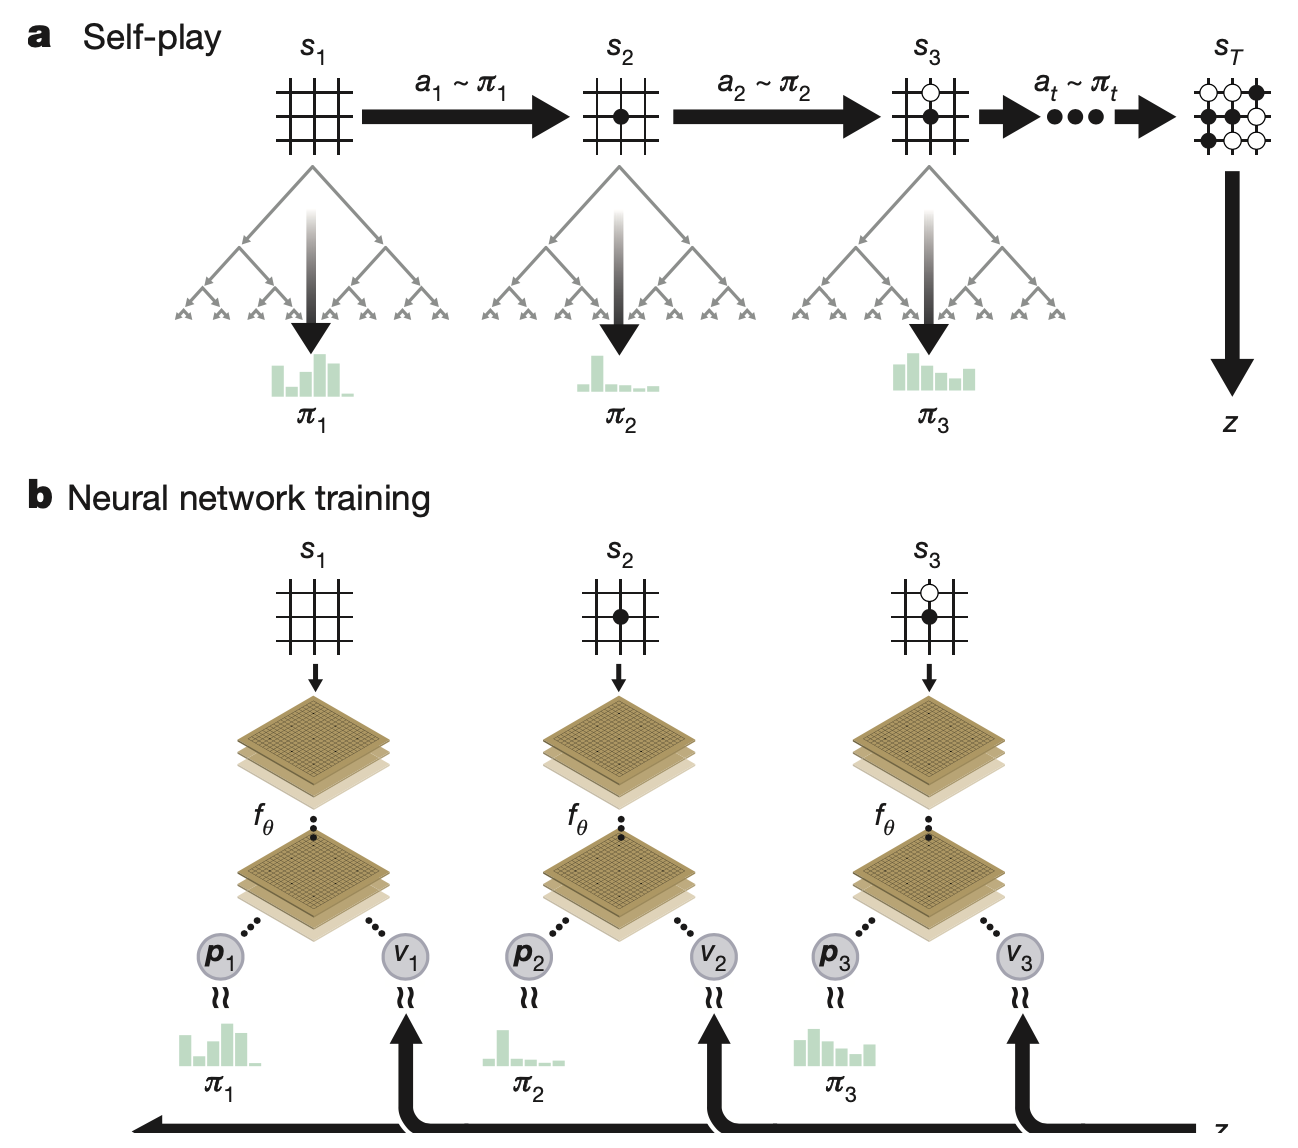
\includegraphics[width=0.4\textwidth]{figures/rl_model_based_alphago_zero_selfplay.png}
		\caption{Self-play RL in AlphaGo zero.}
		\label{fig:rl_model_based_alphago_zero_selfplay}
	\end{figure}
	\item Nevertheless, the training might not be 100\% stable. In a small amount of times, it can happen that the network diverges. To prevent this, we evaluate the network every $n$ steps by playing against itself/an older version of itself. If the policy did not improve (i.e. loosing more games than winning against older version), we throw away the new model and start again from the old weights. 
\end{itemize}